% !TeX root = ../main.tex
% -*- coding: utf-8 -*-
% !TeX root = ../main.tex
% -*- coding: utf-8 -*-


\chapter{绪论}
\label{chpater:introduction}

\section{研究背景}

近年来,随着“双减”政策的全面实施,中国教育领域正在经历一场深刻而全面的变革。传统校外培训行业面临前所未有的转型压力,国家与社会更关注教育质量提升、学生负担减轻,“减负增效”已成为当前教育改革的重要目标。在此背景下,传统的统一化、标准化教育模式逐渐向以学生个性化需求为核心的精准教育模式转型,教育信息化与智能化成为推动教育产业变革的重要引擎。

为积极响应国家政策导向,教育科技企业纷纷开发新的智能化教育产品,如智能学习平板、智能学习伴侣机器人等。其中,根据市场调查机构IDC的数据,2023年中国智能教育硬件市场规模预计达到390亿元人民币,同比增长18.5\%。尤其是以学习行为数据驱动的智能教育产品,由于其能够显著提升学生学习效率与学习效果,逐步成为教育市场竞争的重要方向。

G公司作为国内教育科技领域的领先企业,其智能点阵笔产品是一项典型的创新实践。点阵笔在不改变传统纸笔书写习惯的基础上,通过先进的传感技术实时采集学生的详细笔迹行为数据,并借助人工智能算法进行笔迹识别、实时追踪学生答题过程,实现AI辅助判卷及错题管理。这种个性化学习数据分析方式显著提升了学生学习过程的透明度和教学干预的有效性,成为企业产品差异化竞争的重要优势。

然而,目前教育产品的定价策略仍以成本加成、市场竞争导向定价为主,缺乏对学生个体学习行为特征、知识点掌握状态和支付意愿的深入分析,未能有效实现差异化、动态化的定价服务组合推荐,存在明显的资源错配和收益损失问题。已有研究多集中在通用的定价模型上,鲜有结合具体教育场景、用户行为数据和知识点掌握状态进行深入分析与建模,难以满足实际业务的精准化需求。因此,亟需开展更深入的个性化行为数据驱动的教育产品差异化定价策略研究,构建更为精准有效的资源配置机制,提升企业在教育科技市场的核心竞争力。


\subsection{研究意义}

当前我国教育行业正处于由粗放式、同质化向精细化、个性化发展的关键阶段,智能教育产品与学习数据的快速积累为教育模式与商业模式的双重变革提供了现实基础。然而,围绕教育行为数据的有效利用、用户差异化价值的识别,以及基于学习过程进行个性化服务与定价的机制,相关研究尚处于起步阶段,理论支撑与实证分析均显不足。

在此背景下,本研究聚焦“基于学习行为数据的教育产品差异化组合定价策略”这一具有交叉性质和现实紧迫性的问题,尝试从用户行为建模、知识点掌握状态建模与支付意愿建模的整合视角切入,探索如何构建端到端的个性化差异化定价优化流程。这不仅是对现有教育定价逻辑的延伸与突破,也回应了教育产品如何在保障公平的同时实现资源优化配置与个性化教育服务落地的现实需求。

\textbf{理论意义}:

本研究从行为定价理论与个性化教育场景的融合角度出发,提出以学习行为数据为基础,结合知识点掌握状态与支付意愿,构建差异化组合定价机制,回应当前教育产品在微观层面缺乏数据驱动经济策略与差异化价值挖掘能力的问题。  
通过引入知识点粒度的服务价值建模与端到端优化流程,本研究有助于丰富行为定价理论在教育场景中的应用视角,拓展个性化教育经济学与数据驱动教学决策的研究边界。

\textbf{实践意义}:

从实践层面看,研究成果有助于教育企业基于用户异质性和差异化需求开展更精准的服务组合推荐与定价决策,提升产品转化率与用户满意度,优化平台收益结构。  
另一方面,差异化组合定价机制有助于实现教育产品资源与学生个体学习状态的精准匹配,促进教育资源的公平分配和高效使用,为实现“减负增效”与“精准教学”的政策目标提供理论支撑与技术路径,推动整个教育行业向智能化、个性化与高质量发展方向稳步迈进。

\section{国内外研究现状}

近年来,消费者行为建模、大数据驱动的个性化服务以及动态定价策略逐渐成为学术界与实务界的重要研究方向。尤其在智能教育场景中,如何结合用户行为特征实现精准分群与定价机制的有效匹配,成为交叉领域的热点问题。本文将从国内与国外两个维度梳理已有研究成果,分析其研究路径与方法特征,并指出当前在教育产品定价中的研究空白。

\subsection{国内研究现状}

在国内学术研究中,消费者行为数据与定价策略的结合已有初步探索,主要集中于电商平台与服务型企业。\cite{li_wei_2023} 基于电商用户行为轨迹,提出通过细分用户群体进行行为导向型定价,强调行为数据对价格敏感性判断的重要作用,为平台提升收益与用户满意度提供实证支持。该研究凸显了“行为—价值—定价”之间的可建模关系。

\cite{zhang2022}则将研究聚焦于线下教育培训机构,基于历史支付与学习行为数据优化课程定价结构,其研究验证了差异化价格结构更有助于用户转化率的提升,提示教育场景下用户需求差异应被动态捕捉并反映在价格机制中。与前者相比,该研究强调了定价模型的“动态性”要求。

在方法层面,\cite{meng2023}在智能电网领域引入聚类分析与动态定价联合建模机制,采用自适应分群技术优化响应策略,该框架被广泛认为具备跨行业适应潜力。其创新之处在于:将无监督学习嵌入定价前端策略制定过程,从而增强定价弹性。

\cite{bai2021}以移动互联网App为背景,构建了基于行为聚类的优化定价流程,实证结果表明该策略可提升中长期ARPU值,研究强调定价策略需围绕用户生命周期进行区隔管理,其思想对教育产品具有较强的迁移参考性。

在教育场景下,\cite{wang2021})基于学习者画像提出个性化课程推荐机制,但研究尚未涉及付费行为与价格适配逻辑;\cite{wu2023}强调人机协同下的精准干预机制,通过采集学习过程数据提升服务个性化程度,为基于过程数据的用户分型提供了场景支撑。

综上,国内研究已在用户分群、动态定价与画像生成方面取得一定进展,但大多停留在推荐与资源分配阶段,尚缺乏将学习过程行为与价格机制深度耦合的建模体系。

\subsection{国外研究现状}

在国际研究中,行为经济学与动态定价策略的结合更为成熟,理论模型与实验方法体系较为完善。\cite{ariely2003}提出“coherent arbitrariness”理论,揭示了价格锚定与初始决策路径对用户支付行为的长尾影响,为非理性消费者行为下的定价策略提供了实验支持。该理论为后续基于行为反应的定价优化奠定了理论基础。

\cite{levrini2021}通过神经生理学实验,量化了价格变化在不同用户认知反应中的异质性,说明价格接受度与个体状态显著相关,强化了定价策略中的用户特征建模必要性。

)\cite{goolsbee2002}则在电商平台竞争环境中,研究价格波动与购买行为关系,构建了转化率驱动的行为价格预测模型。该模型揭示了定价与用户行为之间可度量的因果关系,对复杂平台环境下的价格调整具有指导意义。

\cite{nair2007}探讨了跨期价格歧视策略,提出如何根据用户的“支付时机”与“未来学习曲线”设定非均衡价格策略,对具有连续使用性质的教育类产品具有直接启发。\cite{rhee2017}则在垂直差异化产品场景下,分析行为基础上的分层定价机制,明确用户行为数据对定价弹性参数的修正作用。

在教育技术研究中,\cite{nabizadeh2020}系统回顾了学习路径推荐方法,指出行为数据驱动的画像机制是个性化教育核心,但研究更多聚焦于教学匹配而非商业模式建构。\cite{miklosik2020}指出大数据与机器学习在数字营销中正在重塑定价、推荐与广告投放的核心机制,强调构建“预测—反馈—收益”闭环系统的重要性。

综合来看,国外研究在行为驱动定价的理论建构、实验验证及平台应用方面均更为系统,尤其在模型层面已具备“行为特征—支付意愿—收益函数最优化”的完整框架。但相关研究多聚焦于电商、金融、保险等行业,对于教育数据中“学习行为—学习成效—支付行为”之间的交互机制仍研究不足,难以直接迁移应用。

\textbf{小结}:

已有文献充分显示,消费者行为建模与动态定价机制在多个行业场景中已形成较成熟的理论与方法体系,但面向个性化教育产品,尤其是在基于学生学习行为数据与预测成效之上的差异化定价机制,仍缺乏系统研究与实证模型。因此,结合具体教育场景、学习数据特征及用户价值感知机制,构建从行为分型到价格反馈的完整建模链条,既是理论发展的新方向,也是教育智能产品差异化发展的现实需求。
\section{研究内容与方法}

本研究旨在探讨如何基于学生学习行为数据构建精准的学习画像体系,分析用户学习特征、知识掌握状态与支付意愿特征,并在此基础上设计差异化的教育产品组合定价优化策略,提升教育资源配置效率与平台收益能力。研究内容的组织遵循“数据采集—学习画像特征提取—知识掌握状态分析—支付意愿特征分析—差异化组合定价策略设计—策略评估与反馈优化”的逻辑主线展开。

\subsection{研究内容}

本研究聚焦于个性化学习场景下的差异化组合定价优化机制设计,主要包括以下几个方面:

\begin{itemize}
\item \textbf{数据采集与预处理}:基于G公司点阵笔系统所采集的原始数据,包括笔迹行为数据、学习过程数据与答题结果数据,开展数据清洗、缺失处理、归一化等预处理工作;
\item \textbf{学习画像特征提取}:围绕用户学习行为特征,提取学习节奏、笔迹行为、答题表现、跳题行为等关键变量,构建用户画像,反映个体学习特征差异;
\item \textbf{知识掌握状态分析}:基于题目层级的行为数据,评估学生在各知识点的掌握水平,识别其学习瓶颈和潜在弱项,作为精准服务推荐的重要依据;
\item \textbf{支付意愿特征分析}:结合学习表现与行为特征,分析用户对不同价格策略的接受能力,为差异化组合定价策略设计提供参考依据;
\item \textbf{差异化组合定价策略设计}:在学习画像、知识掌握状态与支付意愿特征基础上,设计针对性的教育资源组合推荐与差异化定价策略,提升平台收益与用户满意度;
\item \textbf{策略评估与反馈优化}:通过模拟实验与实际平台数据,对端到端组合定价策略进行效果评估,检验策略在用户转化率、平台收益与用户满意度等方面的综合表现,结合反馈优化学习画像特征提取与策略设计逻辑,完善整体优化流程。
\end{itemize}

\subsection{研究方法与流程}

本研究方法体系遵循“发现问题—分析问题—解决问题”三阶段逻辑主线,具体如图~\ref{fig:tech_route}所示,结合文献研究、数据分析、策略设计与优化评估等方法展开系统研究。

\begin{figure}[htbp]
    \centering
    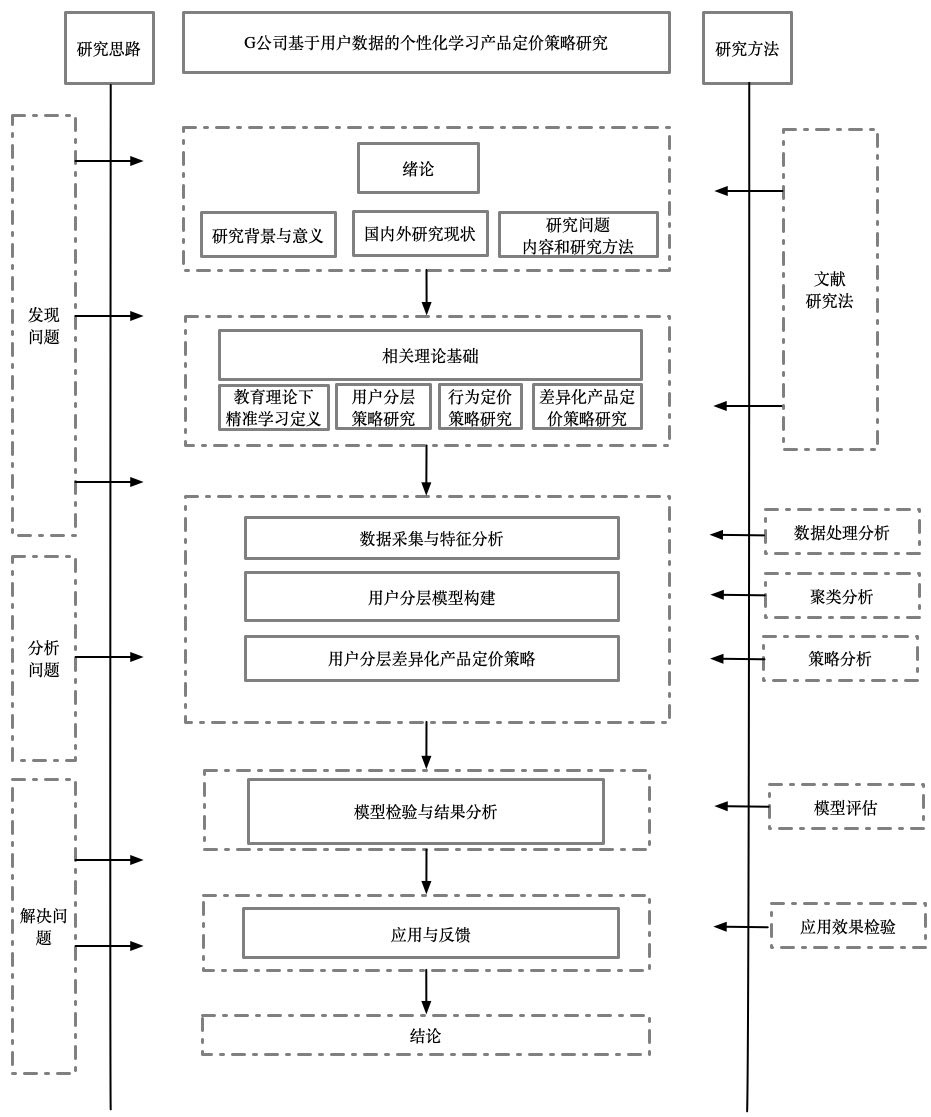
\includegraphics[width=0.8\textwidth]{figure/技术路线图.jpg}
    \caption{本研究的技术路线图}
    \label{fig:tech_route}
\end{figure}

首先在发现问题阶段,通过文献分析法梳理国家政策、教育市场趋势以及个性化学习与差异化定价策略的理论成果,明确当前智能教育产品中定价机制缺乏对学生个体差异、学习状态与支付意愿响应的问题,提出本研究的核心问题与研究思路。

接着在分析问题阶段,从理论与方法层面构建研究框架,界定学习画像特征提取、知识掌握状态分析、支付意愿特征分析与差异化组合定价策略设计的基本思路和实现路径;随后基于点阵笔采集的学习行为数据开展数据处理与特征提取,完成学习画像构建、知识掌握状态分析与支付意愿特征分析,形成差异化组合定价策略设计逻辑。

在解决问题阶段,完成差异化组合定价策略优化的设计与实现,构建端到端优化流程;并通过策略评估方法在实际数据上进行测试,检验组合推荐策略在用户转化率、平台收益与用户满意度等方面的综合表现,结合反馈不断优化学习画像特征提取方法与策略设计逻辑,提升策略效果与实用性。


\section{研究创新}

本研究面向初中数学场景下的教育智能硬件产品,以用户行为数据为基础,构建了一个面向知识点维度、服务内容组合和支付意愿差异的个性化定价模型。相较于传统教育产品的静态定价方式,本研究提出的动态组合式定价方法在理论建模、策略优化与商业应用层面均具有以下创新点:

\begin{itemize}
  \item \textbf{基于行为数据构建多维用户画像,实现行为驱动的动态分群与学习特征刻画。}  
  本研究在G公司智能点阵笔行为数据基础上,提取学习节奏、书写稳定性、题目跳过率、重做次数等多维特征,构建用户学习行为画像。通过K-Means聚类方法,实现了对用户在活跃度、稳定性、行为节奏等维度的自适应划分,替代传统基于静态成绩的用户划分方法,提升了用户价值建模的行为敏感性与时效性。

  \item \textbf{构建了面向知识点的掌握状态量化模型,支撑差异化资源分配与产品策略匹配。}  
  针对初中数学课程中多个核心知识点,设计了一套基于答题正确率、重做率、停顿时长等行为指标的知识点掌握度建模方法。该模型可针对每个用户精细化识别其掌握盲点,为后续产品策略(如推荐哪类教辅资源、引入何种服务)提供基础依据,提升了教育资源分配的精准性。

  \item \textbf{提出了结合用户行为分群与知识掌握状态的个性化服务组合推荐机制。}  
  本研究将用户分群信息与知识点掌握状态共同纳入定价决策机制,根据用户当前掌握情况与行为画像,推荐适配的教辅服务组合(如AI答疑、错题视频讲解、真人1V1答疑等),并考虑不同服务在不同知识点下的价值权重,构建差异化组合策略。这种机制突破了单一服务或定价等级的限制,实现了“用户-知识点-服务”三维匹配的策略设计。

  \item \textbf{构建了基于支付意愿概率的服务定价优化模型,实现收益最大化与策略可解释性的统一。}  
  在定价优化阶段,引入逻辑回归模型对用户支付意愿进行建模,融合用户特征、知识点掌握度与价格敏感度信息,计算不同组合方案下的支付概率。进而在控制服务成本与价格弹性的前提下,求解期望收益最大化的定价策略,形成端到端的个性化定价优化流程,兼顾商业目标与用户接受度。

  \item \textbf{提出了可扩展的组合定价建模框架,具有较强的跨平台与跨学科适应能力。}  
  本研究所提出的“学习行为—知识掌握—支付意愿—组合定价”建模路径,具有较强的模块解耦能力与策略可扩展性。除初中数学场景外,该模型亦可迁移至其他具备行为记录能力的学科或平台(如英语听说系统、科学探究平台等),为后续智能教育产品提供定价机制的通用范式。
\end{itemize}

\section{论文章节}

本文围绕基于学习行为数据的教育产品定价问题,在深入分析个性化教育发展背景及教育科技产品实际应用需求的基础上,结合用户分群建模、学习潜力预测与动态定价机制设计等方法,构建了数据驱动的教育产品定价策略体系,并开展实证验证与策略评估。全文结构安排如下:

第一章 绪论:介绍本研究的背景与意义,说明研究主旨与目标,明确研究内容与方法,回顾国内外相关研究现状,提出本研究的技术路线与论文总体结构。

第二章 理论基础与相关方法:系统阐述个性化教育、行为定价、用户分群与策略建模等相关理论基础,结合聚类分析、行为建模与定价优化等关键技术手段,构建论文研究的理论支撑体系。

第三章 研究内容与技术方法:围绕“发现问题—分析问题—解决问题”的研究主线,详细说明数据采集、特征建模、用户聚类、策略设计与模型评估等研究环节,建立完整的策略构建流程,并结合实际教育数据开展实验建模。

第四章 实证验证与策略评估:基于用户行为数据与平台反馈数据,开展定价策略的效果测试,评估其在提升平台收益、用户接受率与个性化服务水平等方面的表现,验证模型的稳定性、适应性与可推广性。

第五章 研究总结与未来展望:总结本文的主要研究成果与理论贡献,分析当前研究的限制与不足,探讨本研究在更大规模教育平台场景中的扩展潜力,并展望未来行为定价策略在教育智能化发展中的研究前景。


% \begin{itemize}
%   \item 参考文献的录入请参考\ref{sec:relatedwork:ref};
%   \item 图片插入参考\ref{sec:relatedwork:table};
%   \item 分数和公式参考\ref{sec:relatedwork:equation};
%   \item Latex绘图工具参考\ref{sec:method:tikz};
%   \item 代码块参考\ref{sec:method:code};
% \end{itemize}